\section{Efficient architecture}

For building an efficient training architecture, we start by answering the following questions:

\begin{itemize}
    \item What is the family of algorithms that should be supported by this architecture? --- In
    this paper we are aiming to provide a training architecture that will cover model-free
    off-policy and on-policy algorithms with bounded staleness of samples.

    \item What hardware will be used to run the algorithm? --- We consider hybrid CPU/GPU system,
    as it's currently the most widely used platform for training neural networks, and also because
    it provides a good balance between sampling and training performance.

    \item What are the bottlenecks that prevent current algorithms to perform well? --- Most of the
    current algorithms introduce sequential dependency between acting and training procedure, that
    is often absolutely unnecessary and prevents from fully utilizing a hardware and also leads to the
    slowdown when there is a skew in components performance.
\end{itemize}

We address this questions in the new architecture \emph{Decoupled DQN}, that is based on DQN
training procedure, decomposed in a way as to maximize the performance on CPU/GPU system.
Our architecture is shown on Figure \ref{fig:architecture} and consists of three main components:
\begin{itemize}
    \item Actor --- interacts with the environment, by acting and collection the experience. To
        make actions. Uses a separate model replica that is periodically synced with the master replica.
        Runs on CPU, as it doesn't require parallelism or low-latency. Can be scaled up to several
        instances to address slow environment problem.

    \item Trainer --- collects the experience produced by actors and decides which samples will be
        used by learner to train the model. This might include using an internal experience replay
        table or just filtering old samples and forwarding them to the learner.

    \item Learner --- consumes samples provided by trainer to compute gradients and update the
        master model. Runs on GPU, as it needs to perform heavy batch computations.
\end{itemize}

\begin{figure}[h!]
\caption{Decoupled DQN architecture}
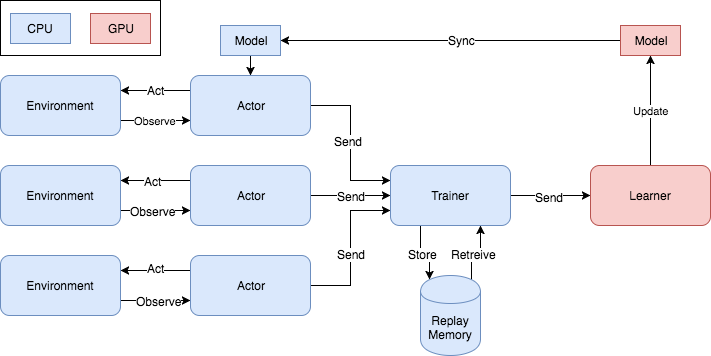
\includegraphics[width=\textwidth]{architecture}
\label{fig:architecture}
\end{figure}

The algorithm \ref{algo:ddqn_algo} shows the pseudo-code for each component thread.
\begin{algorithm}
    \caption{Decoupled DQN}\label{actor}
    \begin{algorithmic}
        \Procedure {Actor}{$env$, $actorQueue$}
            \State $state \gets env.Start()$
            \State $T \gets 0$
            \While{TrainingNotDone}
                \If{$T \mod F_{sync} = 0$}
                    \State $model \gets SyncModel()$
                \EndIf
                \State $action \gets model.Predict(state)$
                \State $nextState, reward \gets env.Act(action)$
                \State $actorQueue.Enqueue(state, action, reward, nextState)$
                \State $state \gets nextState$
                \State $T \gets T + 1$
            \EndWhile
        \EndProcedure
        \Statex
        \Procedure {Trainer}{$actorQueue$, $learnerQueue$}
            \While{TrainingNotDone}
                \State $states, actions, rewards, nextStates \gets actorQueue.Dequeue()$
                \State $StoreExperience(states, actions, rewards, nextStates)$
                \State $learnerQueue.Enqueue(SampleExperience(batchSize))$
            \EndWhile
        \EndProcedure
        \Statex
        \Procedure {Learner}{$learnerQueue$}
            \For{$T \gets 0, T_{max}$}
                \State $batch \gets learnerQueue.Dequeue()$
                \State $Train(batch)$
            \EndFor
        \EndProcedure
    \end{algorithmic}
    \label{algo:ddqn_algo}
\end{algorithm}

We've also experimented with the scheme where actors predictions happen on the GPU, but this
approach trashes the performance of GPU and leads to a worse performance. % graphs?

This architecture has the following advantages:
\begin{itemize}
    \item High utilization for learner hardware. This scheme achieves more then 90\% utilization
        for GPU-based learner allowing it to consume almost 50\% more training samples then DQN in
        the same time.

    \item No sequential blocking of actor and learner. If the environment is very slow, the learner
        can can continue improving the policy and be fully utilized provided the trainer can come up
        with the training examples, which is trivial in case of Q-learning with experience replay.
        We show that the performance of the actor is not influenced by the batch size that is
        used by learner on Figure \ref{fig:batch_size_scalability} (b).
        In contrast, on DQN this blocking leads to the utilization of GPU that has a saw-like
        pattern, and on average is less then 50\%.

    \item Ability to have multiple independent actors that don't interfere with each other. As long
        as there are enough CPU cores on the machine, the actors will be able to run in separate
        threads and achieve linear scalability, as they are using separate copies of the model and
        environment. This model also permits actors that run on multiple machines.

    \item Flexibility in choosing the trainer procedure. We can use schemes with simple forwarding,
        experience replay, or even curriculum learning.
\end{itemize}

Comparing to GORILA architecture, we provide tighter feedback loop, making it possible to use
on-policy algorithms as described in GA3C. Comparing to GA3C each actor leaves in a separate
thread, allowing them to run without introducing the contention and also opening the possibility
to run them on different machines. Our measurements show that running an actor on CPU is only 30\%
slower then running it on GPU, which is a good trade trade-off, as it makes schedule of GPU much
simpler.

\begin{figure*}[!t]
\subfloat[Learner scalability]{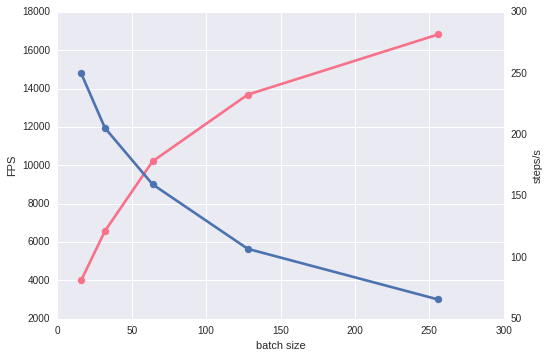
\includegraphics[width=0.5\textwidth]{batch_size_vs_fps_vs_steps}}
\subfloat[Actor isolation]{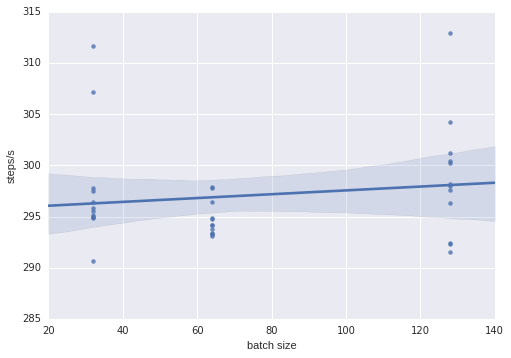
\includegraphics[width=0.5\textwidth]{batch_size_vs_actor_steps}}\\
\caption{Dependence of core system parameters on batch size used by learner. Bigger
batch sizes lead to higher training throughput, and don't influence actors}
\label{fig:batch_size_scalability}
\end{figure*}

We also study the percentage of time spent by the threads in different operations shown
on Figure \ref{fig:ddqn_time} and ensure that learner is spending all the time training.

\begin{figure*}[!t]
\subfloat[Actor]{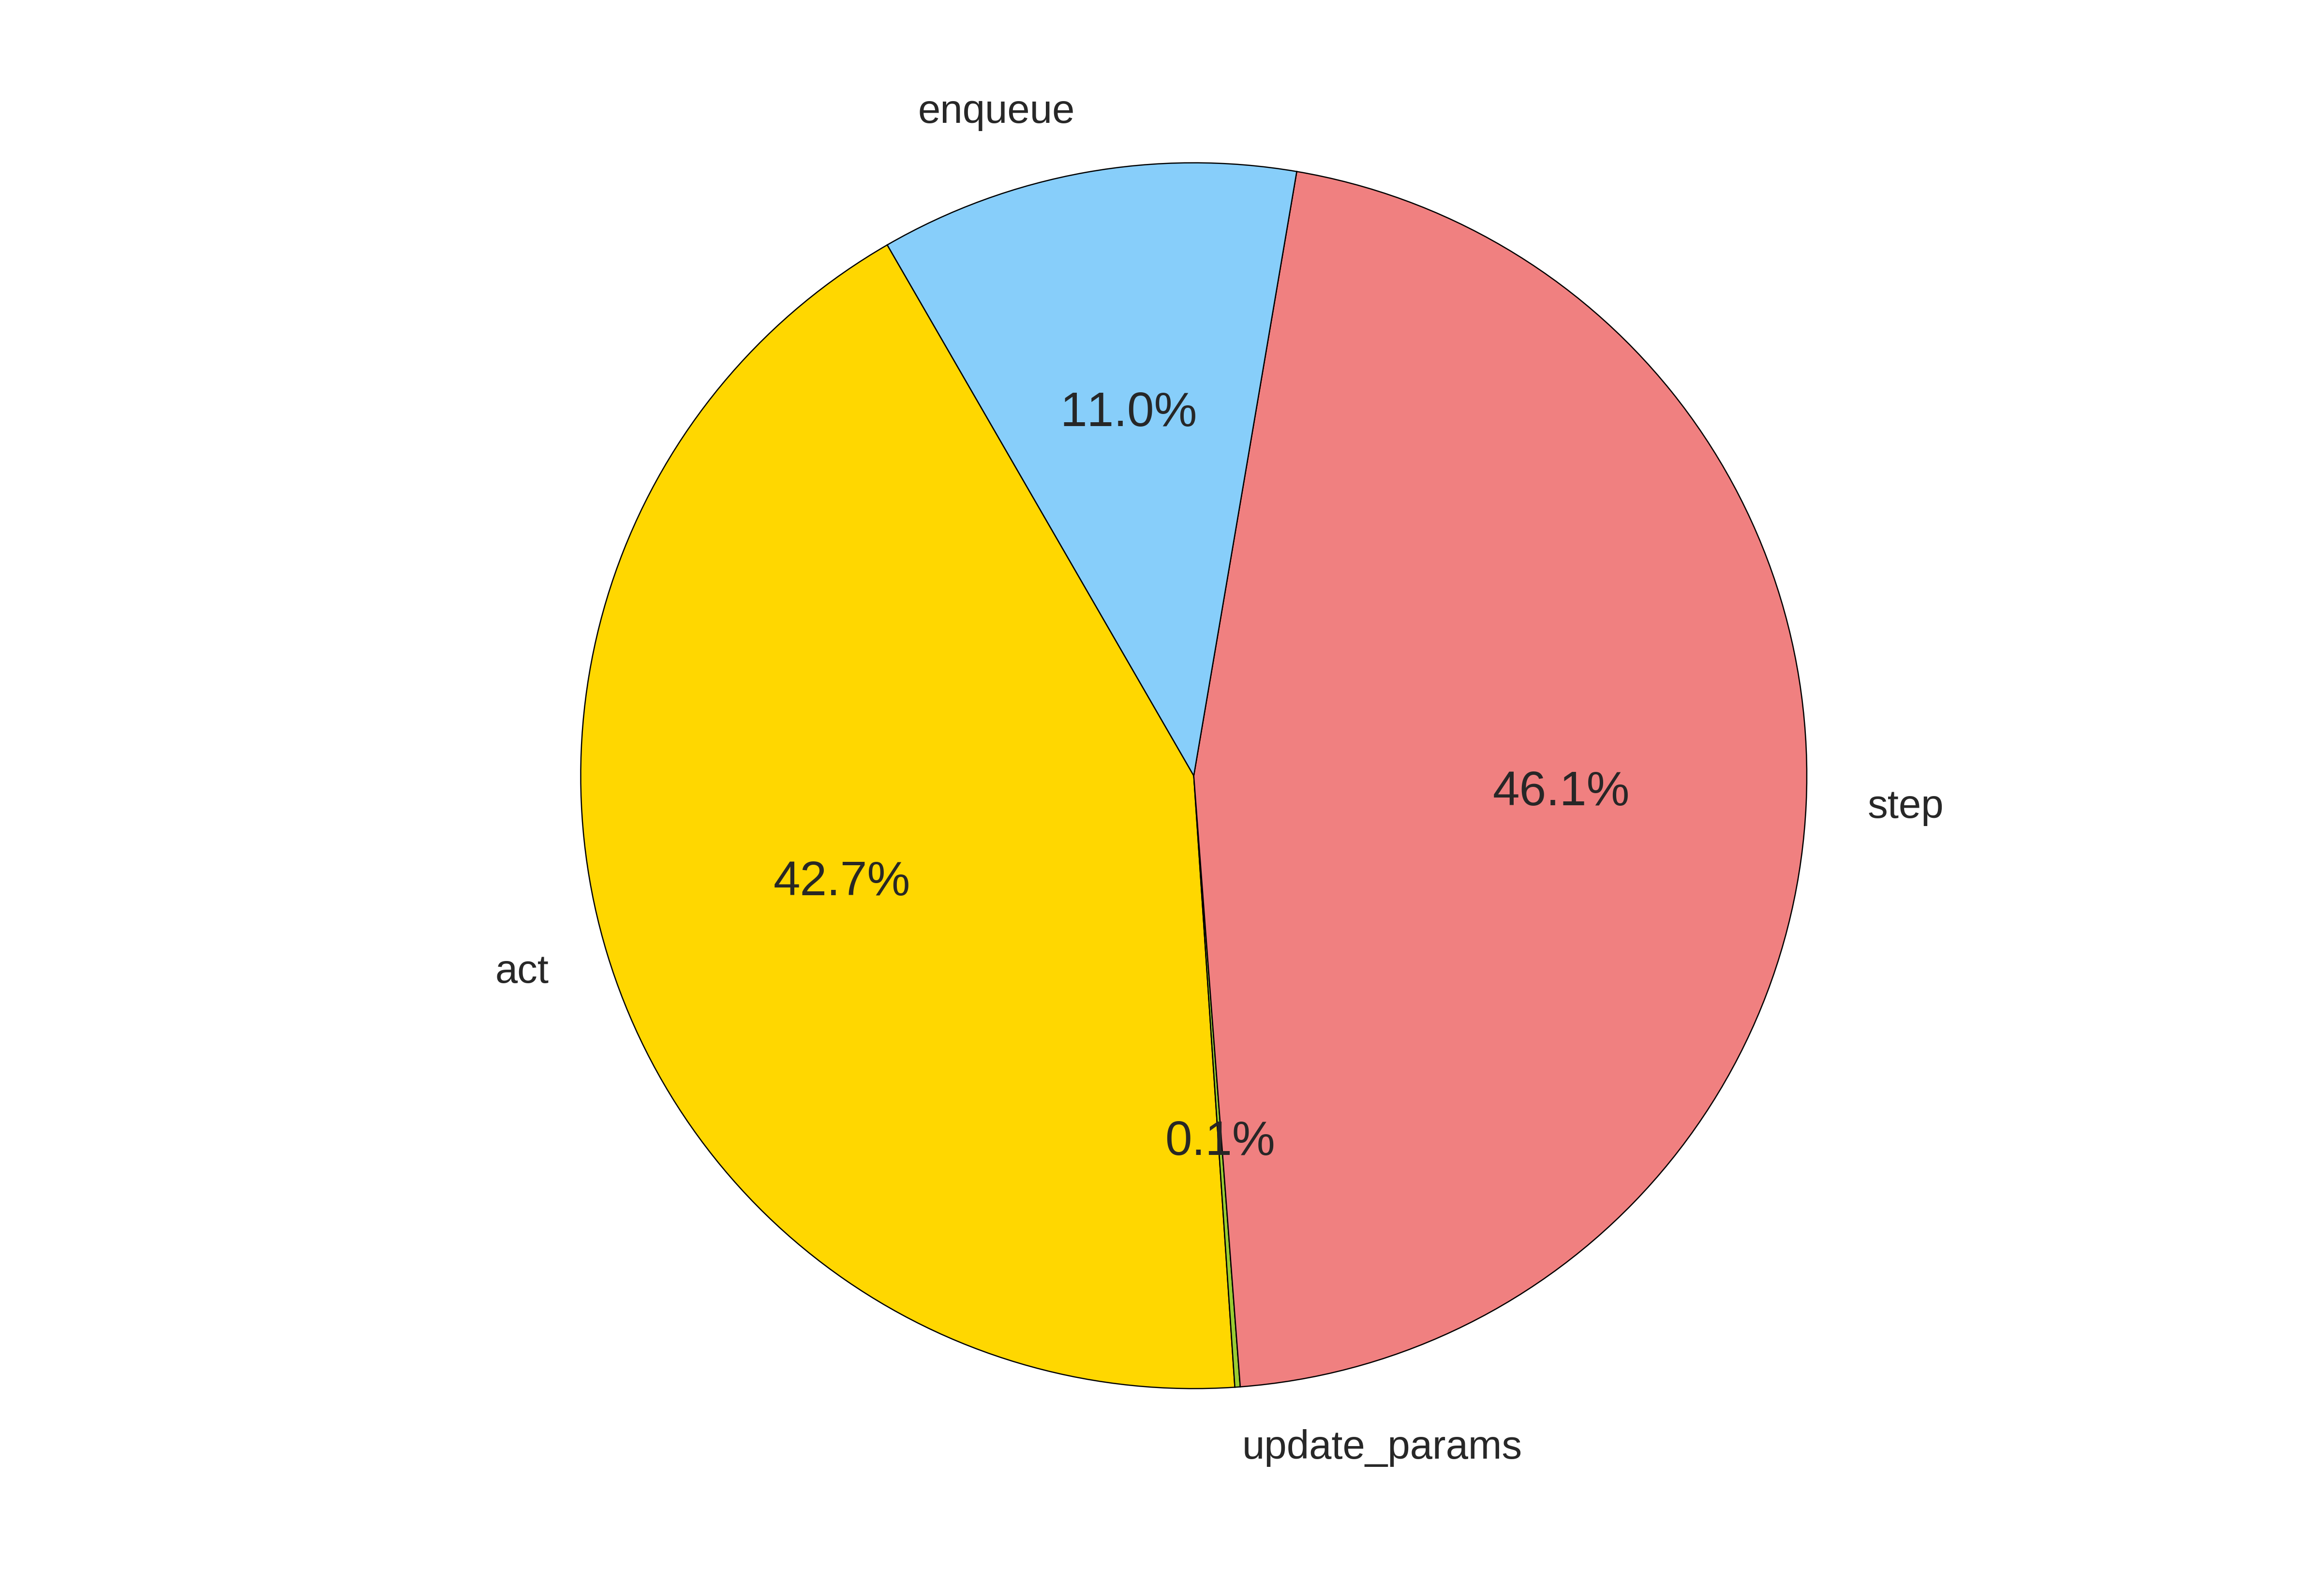
\includegraphics[width=0.5\textwidth]{actor_time_distribution}}
\subfloat[Learner]{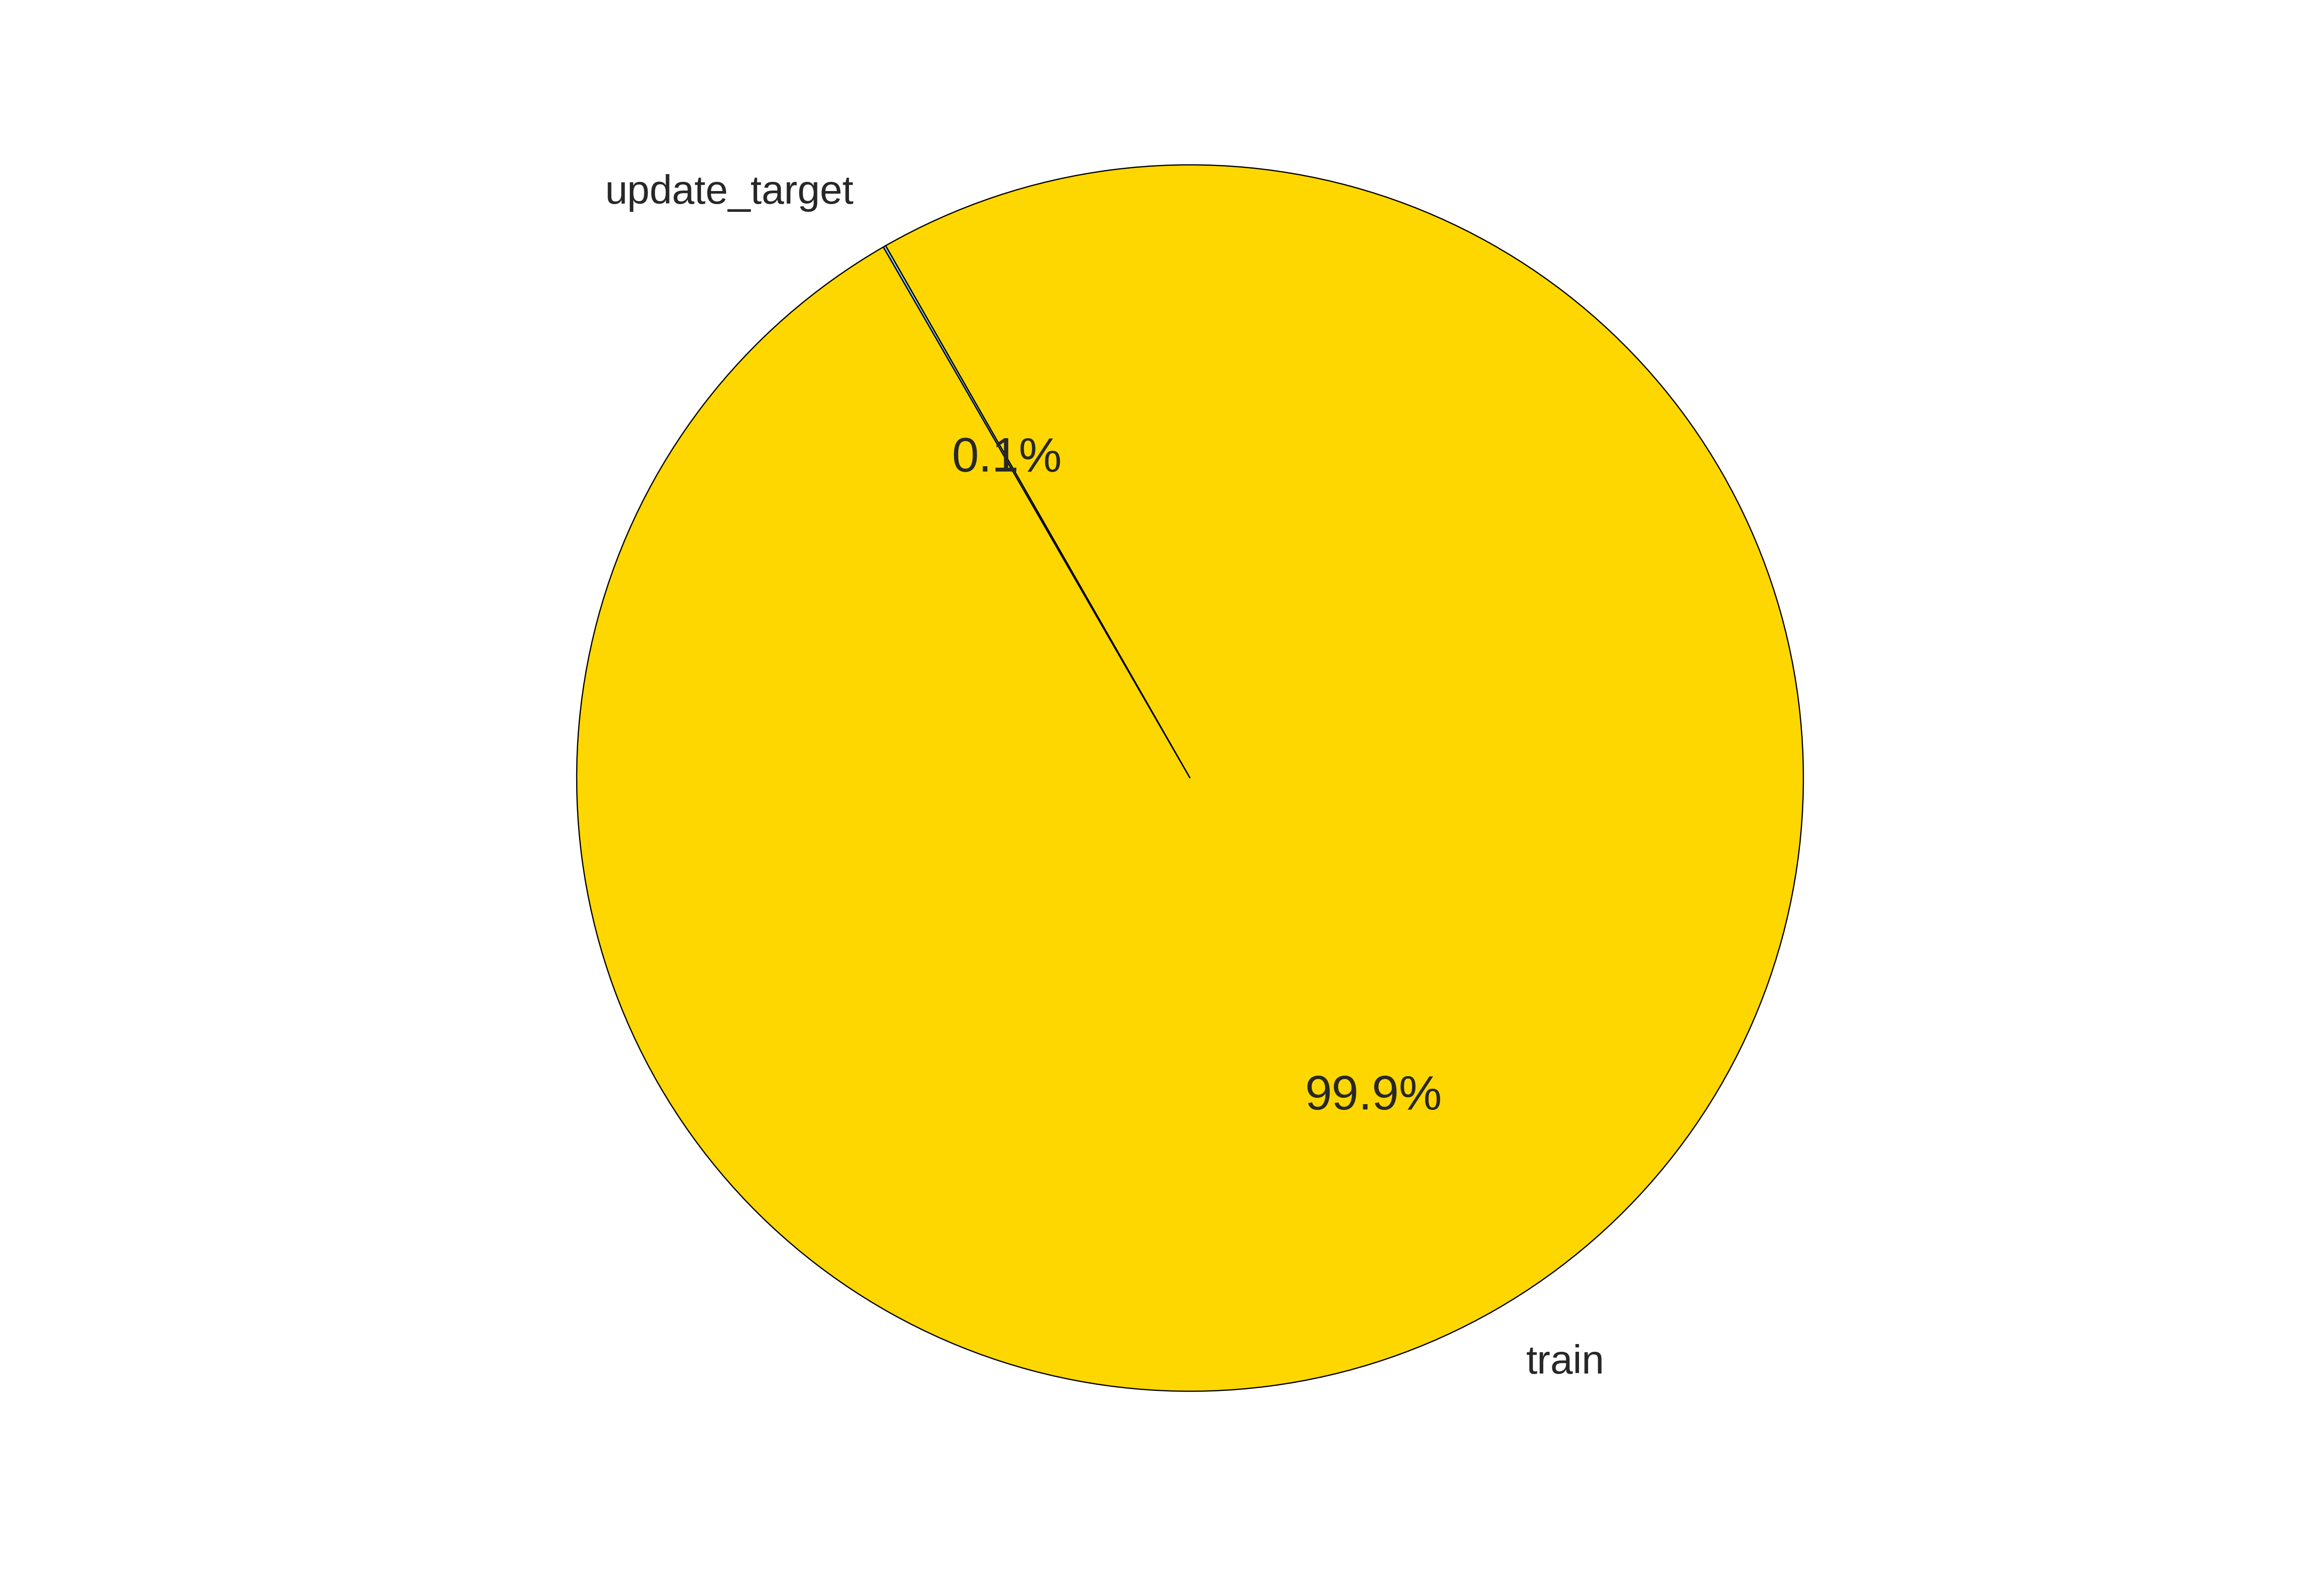
\includegraphics[width=0.5\textwidth]{learner_time_distribution}}\\
\caption{Distribution of Actor and Learner threads time between operations}
\label{fig:ddqn_time}
\end{figure*}

%- Tell about resulting GPU utilization and time spent in different modes of operation.

%- Tell about existing bottlenecks, what will be the limiting factor depending on the env speed,
%training speed, network size.

It's important to note, that this architecture is not limited to Q-learning and can be applied
for on-policy learning in a similar to GA3C way. The challenge there is to ensure that trainer is
not providing too stale samples to the learner, as this might lead to the unstable learning
algorithm.
